% Standard Paper
\documentclass[letterpaper, 10 pt, conference]{ieeeconf}

% A4 Paper
%\documentclass[a4paper, 10pt, conference]{ieeeconf}      

% Only needed for \thanks command
\IEEEoverridecommandlockouts

% Needed to meet printer requirements.
\overrideIEEEmargins

%In case you encounter the following error:
%Error 1010 The PDF file may be corrupt (unable to open PDF file) OR
%Error 1000 An error occurred while parsing a contents stream. Unable to analyze the PDF file.
%This is a known problem with pdfLaTeX conversion filter. The file cannot be opened with acrobat reader
%Please use one of the alternatives below to circumvent this error by uncommenting one or the other
%\pdfobjcompresslevel=0
%\pdfminorversion=4

% See the \addtolength command later in the file to balance the column lengths
% on the last page of the document

% The following packages can be found on http:\\www.ctan.org
\usepackage{graphicx} % for pdf, bitmapped graphics files
%\usepackage{epsfig} % for postscript graphics files
%\usepackage{mathptmx} % assumes new font selection scheme installed
%\usepackage{times} % assumes new font selection scheme installed
%\usepackage{amsmath} % assumes amsmath package installed
%\usepackage{amssymb}  % assumes amsmath package installed

\hyphenation{analysis}

\title{\LARGE \bf HRIStudio: A System for Conducting Human-Robot Interaction Studies using the Wizard-of-Oz Model}

\author{Sean O'Connor and L. Felipe Perrone$^{*}$% <-this % stops a space
%% TODO: Clean up thanks section
    \thanks{$^{*}$Both authors are with the Department of Computer Science,
        Bucknell University, Lewisburg, PA 17837, USA.
            They can be reached at {\tt\small sso005@bucknell.edu} and {\tt\small perrone@bucknell.edu}}%
}

\begin{document}

\maketitle
\thispagestyle{empty}
\pagestyle{empty}


%%%%%%%%%%%%%%%%%%%%%%%%%%%%%%%%%%%%%%%%%%%%%%%%%%%%%%%%%%%%%%%%%%%%%%%%%%%%%%%%
\begin{abstract}

Human-robot interaction (HRI) research plays a pivotal role in shaping how robots communicate and collaborate with humans. However, conducting HRI studies, particularly those employing the Wizard-of-Oz (WoZ) technique, presents challenges due to technical complexities and specialized expertise requirements. To address these challenges, we propose HRIStudio, a novel web-based platform designed to streamline the design, execution, and analysis of WoZ experiments in HRI research. HRIStudio offers an intuitive interface for experiment creation, real-time control and monitoring during live sessions, and comprehensive data logging and playback tools for analysis and reproducibility. By lowering technical barriers and promoting collaboration, HRIStudio aims to accelerate innovation in human-centered robotics research, empowering researchers to explore novel HRI concepts efficiently and effectively.

\end{abstract}


%%%%%%%%%%%%%%%%%%%%%%%%%%%%%%%%%%%%%%%%%%%%%%%%%%%%%%%%%%%%%%%%%%%%%%%%%%%%%%%%


\section{Introduction}

Human-robot interaction (HRI) is an essential field of study for understanding how robots should communicate, collaborate, and coexist with people. The development of autonomous behaviors in social robot applications, however, offers a number of challenges. The Wizard-of-Oz (WoZ) technique has emerged as a valuable experimental paradigm to address these difficulties as it allows experimenters to simulate a robot's autonomous behaviors. With WoZ, a human operator (the \emph{``wizard''}) can operate the robot remotely, essentially simulating its autonomous behavior during user studies. This enables the rapid prototyping and continuous refinement of human-robot interactions postponing to later the full development of complex robot behaviors.

While WoZ is a powerful paradigm, it does not eliminate all experimental challenges. Researchers may face barriers related to the use of specialized tools and methodologies involved in WoZ user studies and also find difficulties in creating fully reproducible experiments. Existing solutions often rely on low-level robot operating systems, limited proprietary platforms, or require extensive custom coding, which can restrict their use to domain experts with extensive technical backgrounds.

Through a comprehensive review of current literature, we have identified a pressing need for a platform that simplifies the process of designing, executing, analyzing, and recording WoZ-based user studies. To address this gap, we are developing \emph{HRIStudio},  a novel web-based platform that enables the intuitive configuration and operation of WoZ studies for HRI research. Our contribution leverages the \emph{Robot Operating System} (ROS) to handle the complexities of interfacing with different robotics platforms. HRIStudio presents users with a high-level, user-friendly interface for experimental design, live control and monitoring, and comprehensive post-study analysis. The system offers drag-and-drop visual programming for describing experiments without extensive coding, real-time control and observation capabilities during live experiment sessions, as well as comprehensive data logging and playback tools for analysis and enhanced reproducibility. We expect that with these features, HRIStudio will increase the usability of the  WoZ paradigm and increase scientific rigor of HRI experiments. The following sections outline our proposed system design, experimental workflow structure, implementation progress, and future directions for this work.

\section{State-of-the-Art}

The importance of the WoZ paradigm for user studies in social robotics is illustrated by the 
several frameworks that have been developed to support it. We describe here some of the most notable.

Polonius \cite{Lu2011} offers a graphical user interface for wizards to control robots based on predefined finite state machine scripts. While built on the modular ROS platform, Polonius lacks enhanced tools for experiment design, data analysis, and cross-platform collaboration. NottReal \cite{Porcheron2020}, designed for voice user interface research, provides scripting capabilities and visual feedback to enhance the illusion of autonomy for participants. However, its scope is limited to audio-based interactions.

WoZ4U \cite{Rietz2021} presents a user-friendly GUI that makes HRI studies more accessible to non-programmers. The tight hardware focus on Aldebaran's Pepper, however, constrains the tool's applicability. OpenWoZ \cite{Hoffman2016} proposes a runtime-configurable framework with a multi-client architecture, enabling evaluators to modify robot behaviors during experiments. OpenWoZ promotes standardization, but requires programming expertise for customization. A systematic review by Reik \cite{Riek2012} highlights prevalent WoZ applications in natural language processing and non-verbal behavior simulation but identifies gaps in methodological rigor, such as lack of wizard training and error measurement. The review proposes reporting guidelines to enhance transparency and reproducibility in WoZ studies.

These efforts have inspired us to pursue the consolidation of their various features into a new tool that offers more comprehensive support for Woz Experiments in social robotics. In the conceptualization of HRIStudio, we have aimed to incorporate an intuitive GUI, support for a broader range of robots, mechanisms for describing WoZ experiments, and the centralized aggregation of results and experimental data to enable easier collaboration, dissemination, and reproduction. 
 
\section{Experimental Workflow}

\subsection{Experimental architecture}

We propose a hierarchical organization of experimental elements to provide a structured framework for designing WoZ experiments in HRI research. At the highest level, an \textit{experiment} represents the complete scientific study being conducted. Within each experiment, researchers can define a series of \textit{steps}, which represent conceptual stages or phases of the experimental protocol. These \textit{steps} serve as logical containers for grouping and sequencing the specific \textit{actions} that the robot or the wizard must perform throughout the duration of the study, as illustrated in Figure \ref{experimentalarchitecture}.

\begin{figure}[ht]
   \vskip -0.3cm
    \begin{center}
        \includegraphics[width=0.4\paperwidth]{assets/diagrams/experimentalarchitecture}
        \vskip -0.5cm
        \caption{A sample experiment examining comprehension over varying modes of interaction}
        \label{experimentalarchitecture}
    \end{center}
\vskip -0.3cm
\end{figure}

At the lowest level, \textit{actions} constitute the elemental units of the experimental workflow. Each \textit[action] corresponds to a specific physical or virtual task that the robot or wizard must execute. These tasks encompass a spectrum of activities, including robot movements, verbal interactions, or awaiting participant input.

By breaking down the experimental procedure into this hierarchical structure, researchers can design complex HRI studies while maintaining a clear set of instructions for each wizard. The \textit{steps} provide a high-level overview of the experimental phases, while the \textit{actions} encapsulate the granular tasks and behaviors required from the robot or the wizard.

\subsection{Experiment creation process}

To enable intuitive and streamlined experiment design, our platform features a user-friendly interface for creating and configuring WoZ experiments in HRI research. This interface leverages a visual programming system, allowing researchers to construct their experiments using a drag-and-drop approach.

The core of the experiment creation process will include a library of pre-defined action components, representing common tasks and behaviors that robots and wizards may need to perform during an experiment, including robot movements, speech synthesis, and instructions for the wizard. Researchers are able to drag and drop these action components onto a canvas, arranging them into sequences that define the steps of their experiment. Each step can contain one or more actions, enabling the construction of complex experimental protocols.

In addition to arranging actions and steps, the interface will provide configuration options for each component, allowing researchers to go beyond the pre-defined action library to customize parameters. This configuration system will be accompanied by contextual help and documentation, guiding researchers through the process and providing examples or best practices for designing functional experiments.

\subsection{Live experiment operation}

During live experiment sessions, our platform offers multiple synchronized views to streamline operation, observation, and data collection. The primary view, tailored for the wizard, enables seamless control over the robot's actions and behaviors. Displaying the current step of the experiment along with associated actions, this interface facilitates intuitive navigation and note-taking. The wizard can progress through actions sequentially or manually trigger specific actions based on contextual cues or participant responses. Additionally, controls for robot movements, speech synthesis, and other essential functions are readily accessible.

In parallel, the observer view supports live monitoring, note-taking, and potential interventions by additional researchers or personnel involved in the experiment. This feature ensures the option of continuous oversight without disrupting the participant's experience or the wizard's control. Given the web-based nature of our platform, multiple observers can concurrently access the observer view, enhancing collaboration and enabling comprehensive data collection and analysis.

\subsection{Data logging, playback, and annotation}

Throughout the live experiment session, the platform will automatically log various data streams, including timestamped records of all executed actions and experimental events, exposed robot sensor data, and audio and video recordings of the participant's interactions with the robot. This logged data will be stored in JavaScript Object Notation (JSON) files kept in a secure encrypted location, enabling efficient post-experiment analysis and data mining without compromising the privacy of the subjects or researchers.

After an experiment session, researchers will have access to a dedicated playback interface. This interface will allow them to review the recorded data streams synchronously, enabling a holistic understanding of the experiment's progression. This interface will support features such as: synchronized playback of audio, video, and sensor data streams, visual annotations and note taking capabilities, navigation and scrubbing through the recorded data with the ability to mark and note significant events or observations, and export options for selected data segments or annotations.

By providing robust data logging and playback capabilities, our platform aims to enhance the rigor and reproducibility of HRI WoZ experiments.


\section{Proposed System Design}

\subsection{High-level architecture}

We have designed our system as a full-stack web application using the \emph{Next.js React} framework. The frontend handles the user interface components like the experiment designer, monitoring dashboard, and analysis tools. The backend API logic, built using Next functions and tRPC, manages experiment data, user authentication, and communication with a ROS interface component. The ROS interface, implemented as a separate C++ node, translates high-level actions from the web application into low-level robot commands, sensor data, and protocols, abstracting the complexities of different robotics platforms. This modular architecture aims to leverage the benefits of Next's server-side rendering, improved performance, and security, while enabling integration with various robotic platforms through ROS.

\begin{figure}[ht]
   \vskip -0.3cm
    \begin{center}
        \includegraphics[width=0.4\paperwidth]{assets/diagrams/highlevelarchitecture}
        \vskip -0.3cm
        \caption{The high-level system architecture of HRIStudio}
        \label{highlevelarchitecture}
    \end{center}
     \vskip -0.4cm
\end{figure}

\subsection{Key design principles}

In developing this novel platform for WoZ experiments in HRI research, we have identified several guiding design principles to ensure its effectiveness, usability, and widespread adoption.

Foremost, simplicity and accessibility are of the highest priority. Our primary objective is to lower the barrier of entry for non-programming domain experts who wish to conduct HRI studies. The platform will provide an intuitive and user-friendly interface, abstracting users from the intricacies of robot programming and autonomous system development.

Furthermore, our design principles prioritize reproducibility and collaboration. To achieve these objectives, we foster scientific integrity through extensive experiment logging and seamless export and sharing functionalities.

Additionally, our platform embraces a hardware-agnostic approach. Leveraging a modular and extensible architecture, it seamlessly integrates with a wide array of consumer and research robots through the ROS interface, ensuring compatibility with already available hardware.


\section{IMPLEMENTATION PROGRESS}

While the full realization of the proposed platform is still a work in progress, we have made notable strides in several key areas to lay the groundwork for its development. Our efforts thus far have primarily focused on exploring the core technologies, creating user interface mockups, and establishing a development roadmap.

\subsection{Core technologies}

We have chosen to leverage the Next.js React framework for building the web application element of our platform. Next provides several advantages, including server-side rendering, improved performance, and enhanced security compared to traditional single-page applications. With the application being available on the web, we aim to provide compatibility with most hardware currently available to researchers. Additionally, the framework's built-in support for API routes and its ability to integrate with tRPC will simplify the development of APIs for interfacing with the ROS interface.

For the robot control layer, we plan to utilize ROS as the communication and control interface. ROS offers a modular and extensible architecture, enabling seamless integration with a multitude of consumer and research robotics platforms. By leveraging the widespread adoption of ROS in the robotics community, our platform aims to support a wide range robots out-of-the-box, with the support of the already existing ROS community available for new robot implementations.

\subsection{User interface mockups}

A significant portion of our efforts have been dedicated to designing intuitive and user-friendly interface mockups for the platform's key components. We have created wireframes and prototypes using Figma for the frontend's dashboard, drag-and-drop experiment designer, the real-time experiment monitoring and control dashboard, and the data playback and annotation tools.

The project dashboard mockups (see Figure \ref{dashboard}) display an intuitive overview of a project's status, including platform information, collaborators, completed and upcoming trials, subjects, and a list of pending issues. This will allow a researcher to quickly see what needs to be done, or easily navigate to a previous trial's data for analysis.

\begin{figure}[h]
    \begin{center}
        \includegraphics[width=0.4\paperwidth]{assets/mockups/projectdashboard}
        \vskip -0.3cm
        \caption{A sample project dashboard within HRIStudio}
        \label{dashboard}
    \end{center}
    \vskip -0.4cm
\end{figure}

The experiment designer mockups depicted in Figure \ref{designer} feature a visual programming canvas where researchers can construct their experiments by dragging and dropping pre-defined action components. These components represent common tasks and behaviors, such as robot movements, speech synthesis, and instructions for the wizard. The mockups also include configuration panels for customizing the parameters of each action component.

\begin{figure}[h]
    \begin{center}
        \includegraphics[width=0.4\paperwidth]{assets/mockups/experimentdesigner}
         \vskip -0.3cm
        \caption{A sample project's designer view in HRIStudio}
        \label{designer}
    \end{center}
    \vskip -0.5cm
\end{figure}

For the live experiment operation, we have designed mockups that provide synchronized views for the wizard and observers. The wizard view (see Figure \ref{wizardview}) presents an intuitive step-based interface that walks the wizard through the experiment as specified by the designer, triggering actions, and controlling the robot, while the observer view facilitates real-time monitoring and note taking.

\begin{figure}[h]
    \begin{center}
        \includegraphics[width=0.4\paperwidth]{assets/mockups/wizardview}
         \vskip -0.3cm
        \caption{The wizard's view during a live experiment}
        \label{wizardview}
    \end{center}
    \vskip -0.5cm
\end{figure}

Our data playback and annotation mockups (showcased in Figure \ref{playback}) showcase features for synchronized playback of recorded data streams, including audio, video, and applicable sensor data. These mockups incorporate visual and textual annotations, scrubbing capabilities, and data export options to support comprehensive post-experiment analysis and reproducibility.

\begin{figure}[h]
    \begin{center}
        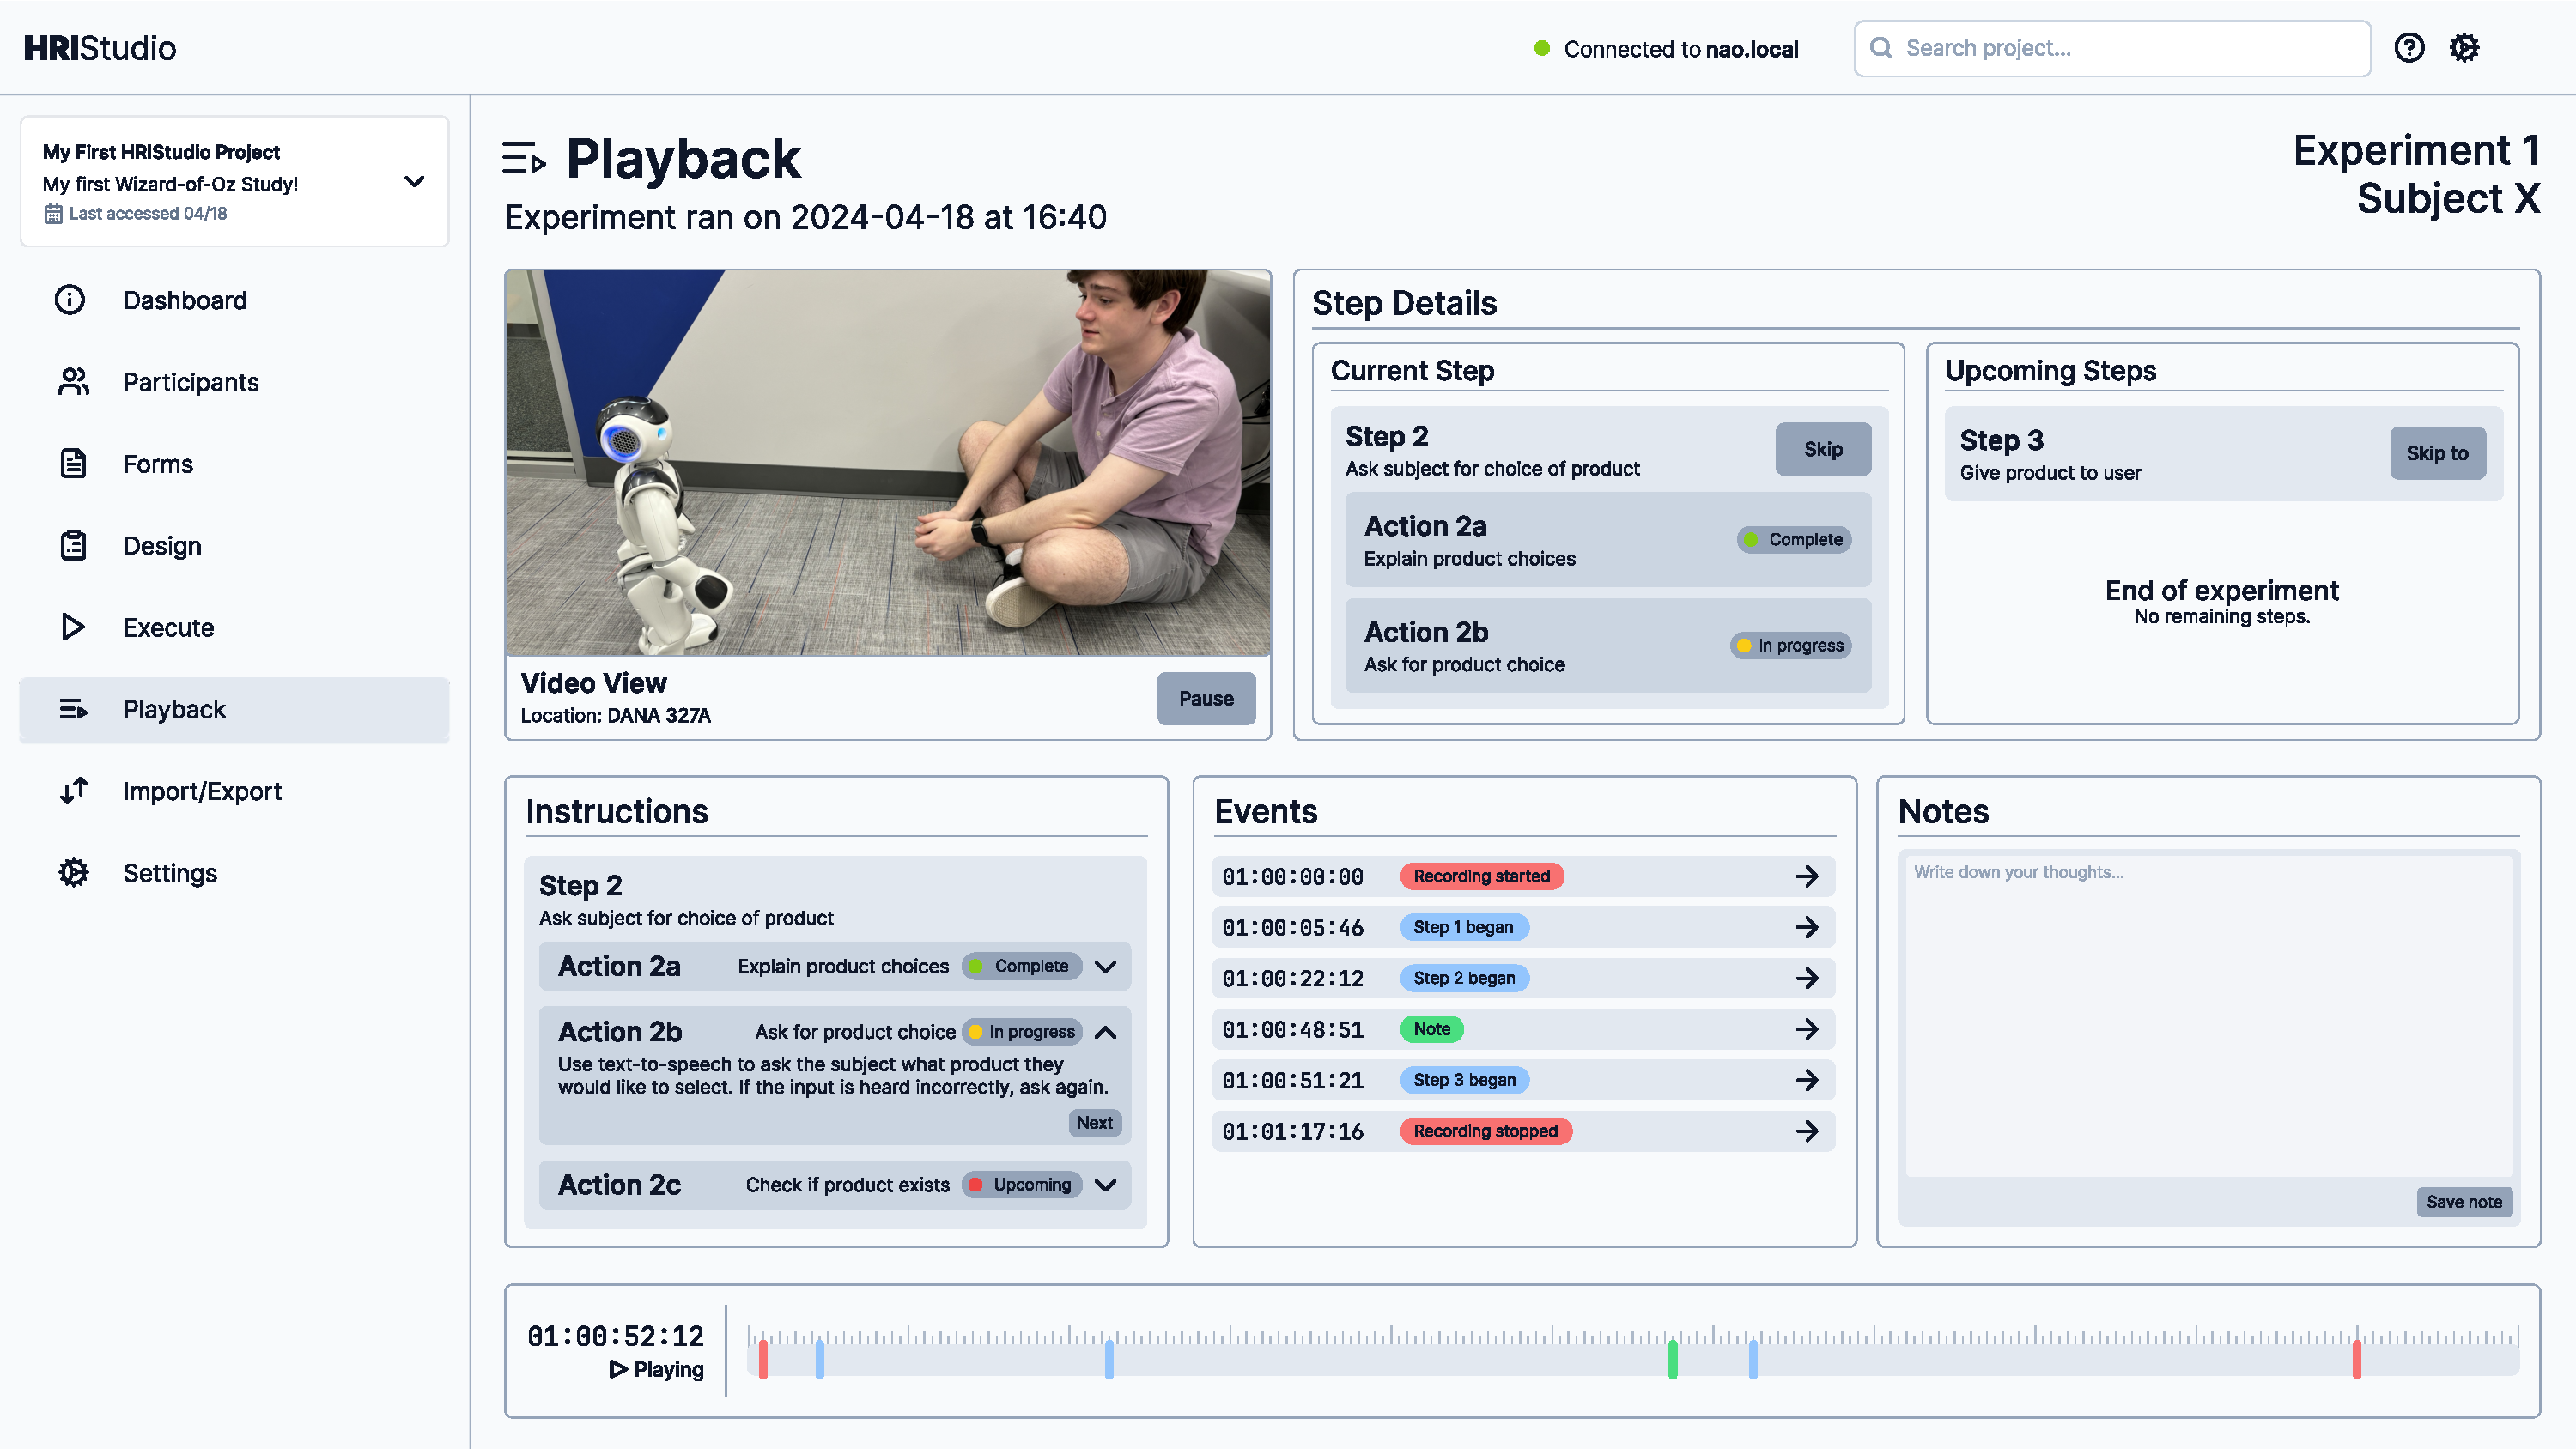
\includegraphics[width=0.4\paperwidth]{assets/mockups/playback}
         \vskip -0.3cm
        \caption{The playback view of an experiment's trial}
        \label{playback}
    \end{center}
    \vskip -0.7cm
\end{figure}

\subsection{Development roadmap}

While the UI mockups have laid a solid foundation, we still anticipate several challenges in transforming these designs into a fully functional platform. One of the primary challenges will be integrating the Next web application with the ROS interface, and handling the bi-directional communication between the two systems. We anticipate leveraging tRPC and WebSockets to facilitate real-time data exchange and robot control.

Another significant challenge lies in developing the drag-and-drop experiment designer and encoding the experimental procedures into a standardized, shareable format. We plan to explore existing visual programming libraries and develop custom components to enable intuitive experiment construction and configuration.

Additionally, implementing robust data logging and playback capabilities will require integrating with various data streams, such as audio, video, and sensor data, while ensuring synchronization and efficient storage and retrieval mechanisms.

%% TODO: Consolidate roadmap, consider replacing with future challenges/work.

To address. these challenges, our development roadmap includes:
\begin{itemize}
    \item Establishing a stable Next codebase and integrating tRPC for API development.
    \item Implementing a C++ ROS node for handling robot communication and control.
    \item Developing the drag-and-drop experiment designer using visual programming libraries and custom components.
    \item Integrating data logging mechanisms for capturing experimental data streams.
    \item Building the data playback and annotation tools with synchronization and export capabilities.
    \item Documenting the platform and creating tutorials and guidelines for researchers to adopt and contribute to the system.
\end{itemize}

By following this roadmap and addressing the identified challenges, we aim to transform the proposed platform into a fully functional and accessible tool for conducting WoZ experiments in HRI research, empowering researchers and fostering collaboration within the community.

%\section*{APPENDIX}
%
%% TODO: Complete appendix
%Appendixes should appear before the acknowledgment.
%
%\section*{ACKNOWLEDGMENT}
%
%% TODO: Make acknowledgments
%The preferred spelling of the word acknowledgment in America is without an e after the g. Avoid the stilted expression, One of us (R. B. G.) thanks . . .  Instead, try R. B. G. thanks. Put sponsor acknowledgments in the unnumbered footnote on the first page.

\bibliography{refs}
\bibliographystyle{plain}

\end{document}
